\documentclass{standalone}
\usepackage{tikz}
\usepackage{ctex,siunitx}
\setCJKmainfont{Noto Serif CJK SC}
\usepackage{tkz-euclide}
\usepackage{amsmath}
\usetikzlibrary{patterns, calc}
\usetikzlibrary {decorations.pathmorphing, decorations.pathreplacing, decorations.shapes,}

\begin{document}
\small
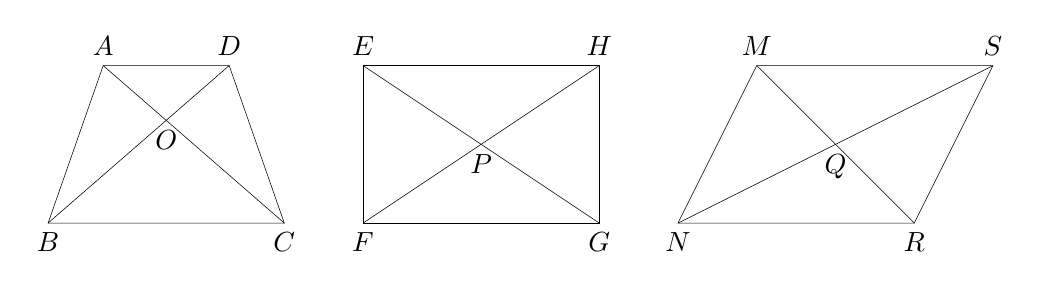
\begin{tikzpicture}[>=stealth,scale=1]
  \tkzSetUpPoint[fill=black]
  % \useasboundingbox(-1,-0.75)rectangle(3.7,1.4);
  \begin{scope}
  \tkzDefPoints{-1.5/0/B, 1.5/0/C, -.8/2/A, .8/2/D}
  \tkzDrawPolygon(A,B,C,D)
  \tkzInterLL(A,C)(B,D)  \tkzGetPoint{O}
  \tkzLabelPoints[below](B,C,O)
  \tkzLabelPoints[above](A,D)
  \tkzDrawSegments(A,C B,D)
  \end{scope}
  \begin{scope}[xshift=4cm]
  	\tkzDefPoints{-1.5/0/F, 1.5/0/G, -1.5/2/E, 1.5/2/H}
  \tkzDrawPolygon(E,F,G,H)
  \tkzInterLL(E,G)(F,H)  \tkzGetPoint{P}
  \tkzLabelPoints[below](F,G,P)
  \tkzLabelPoints[above](E,H)
  \tkzDrawSegments(E,G F,H)
  \end{scope}
  \begin{scope}[xshift=8cm]
  	\tkzDefPoints{-1.5/0/N, 1.5/0/R, 2.5/2/S, -.5/2/M}
  \tkzDrawPolygon(M,N,R,S)
  \tkzInterLL(M,R)(N,S)  \tkzGetPoint{Q}
  \tkzLabelPoints[below](N,R,Q)
  \tkzLabelPoints[above](M,S)
  \tkzDrawSegments(M,R N,S)
  \end{scope}
\end{tikzpicture}
\end{document}